\documentclass[12pt]{article}
\usepackage[margin=1in]{geometry}
\usepackage{subcaption}
\usepackage{graphicx}
\usepackage{gensymb}
\usepackage{amssymb}
\usepackage{amsmath}
\usepackage{units}
\usepackage{graphicx}
\usepackage{listings}
% \usepackage{setspace}o
% \onehalfspacing
% \usepackage[english]{babel}
% \usepackage[utf9]{inputenc}
% \pagestyle{headings}

\title{Computational Practicum report}
\author{Latypov Daniil BS20-01}
\date{}

\begin{document}
\maketitle
\section*{Analytical solution}
\subsection*{General solution}
The following differential equation is given:
\begin{gather}
y'=\frac{4}{x^2} - \frac{y}{x} - y^2
\end{gather}
The domain of x is $x \in \mathbf{R} \backslash \{0\}$. \\
Equation can be rewritten in the following way:
\begin{gather*}
    y'+(- \frac{1}{x})y + ( -1 ) y^2 = \frac{4}{x^2}
\end{gather*}
From this we can see, that the equation is a Ricatti equation. \\
We suppose that $y = y_2 + u(x)$, $y_1 = \frac{a}{x}$. Then $y_1' = - \frac{a}{x^2}$. \\ 

Substituting $y=y_1$ into (1), we get:
\begin{gather*}
- \frac{a}{x^2} = \frac{4}{x^2} - \frac{a}{x^2} - \frac{a^2}{x^2}
\end{gather*}
From this equation we can easily find $a=2$. \\
Then, $y_1 = \frac{2}{x}$. $y = \frac{2}{x} + u(x)$,
$y' = - \frac{2}{x^2} + u'(x)$

Substituting into (1) we get:
\begin{gather*}
- \frac{2}{x^2} + u' = - \frac{2}{x^2} - \frac{u}{x} - \frac{4}{x^2} - u^2\
- \frac{4u}{x} + \frac{4}{x^2}
\end{gather*}
Which is equivalent to:
\begin{gather}
u'= -u^2 - \frac{5u}{x}
\end{gather}
Then, with the use of substitution $ u = \frac{1}{z}$, 
$u'= - \frac{1}{z^2}z'$ we get:
\begin{gather*}
- \frac{z'}{z^2} + \frac{5}{zx} = - \frac{1}{z^2}
\end{gather*}

Multiplying both sides by $z^2$ and rewriting we get the following equation:
\begin{gather}
z' = 1 + \frac{5z}{x} 
\end{gather}
It's complementary equation can be written as:
\begin{gather*}
\frac{1}{z}dz = \frac{5}{x}dx
\end{gather*}
Taking integral of both sides:
\begin{gather*}
ln|z| = 5ln|x|
\end{gather*}
Therefore, 
\begin{gather}
    z = x^5 * C_1
\end{gather}
Where $C_1 = C_1(x)$, $ z'= 5x^4*C_1 + x^5*C_1'$. \\
Substituting into (3), we get:
\begin{gather*}
5x^4*C_1 + x^5*C_1' = \frac{x^5 * C_1 }{x} - 1
\end{gather*}
From this we find:
\begin{gather*}
x^5 * C_1' = -1 \Rightarrow C_1 = \frac{1}{4x^4} + C_2
\end{gather*}
Substituting into (4) we get:
\begin{gather*}
z = - \frac{x}{4} + x^5*C_2
\end{gather*}
Backsubstituting $ z= \frac{1}{u}$ we get:
\begin{gather*}
u = \frac{1}{ -\frac{x}{4} + x^5*C_2 } \Rightarrow u = \frac{4}{4x^5*C_2 - x}
\end{gather*}
Backsubstituting $ y = \frac{2}{x} + u$ we get the general solution on 
domain $x \in \mathbf{R} \backslash \{0\}$, \\
where $4C*x^5 - \frac{x}{4} \neq 0$:
\begin{gather*}
y = \frac{2}{x} +  \frac{4}{ 4C*x^5 - x }
\end{gather*}
\subsection*{Initial value problem}
Solving the Initial value problem:
\begin{gather*}
0 = 2 + \frac{4}{4C-1} \Rightarrow C = -\frac{1}{4}
\end{gather*}
Therefore, the particular solution is:
\begin{gather*}
y = \frac{2}x + \frac{4}{-x -x^5}
\end{gather*}
\newpage
\subsection*{Analysis of points of discontinuity}
From the general solution we can express C 
\begin{gather*}
    C = \frac{1}{x_0^4} \Bigg( \frac{1}{x_0y_0-2} + 1 \Bigg)
\end{gather*}
If $C = 0$, then there is only one point of discontinuity, $x=0$. \\
If $C \neq 0$, then there are 3 points of discontinuity, that can be found
in the following way:
$$
\begin{cases}
        x \neq 0, \\
        4C*x^5 - x \neq 0
\end{cases}
\Rightarrow
\begin{cases}
        x \neq 0, \\
        x \neq \pm \sqrt[4]{ \frac{1}{4C} }
\end{cases}
$$

\newpage
\section*{Code}
\subsection*{UML Diagram}

The following diagram shows the class structure of my program.
It follows the model-view-controller pattern.

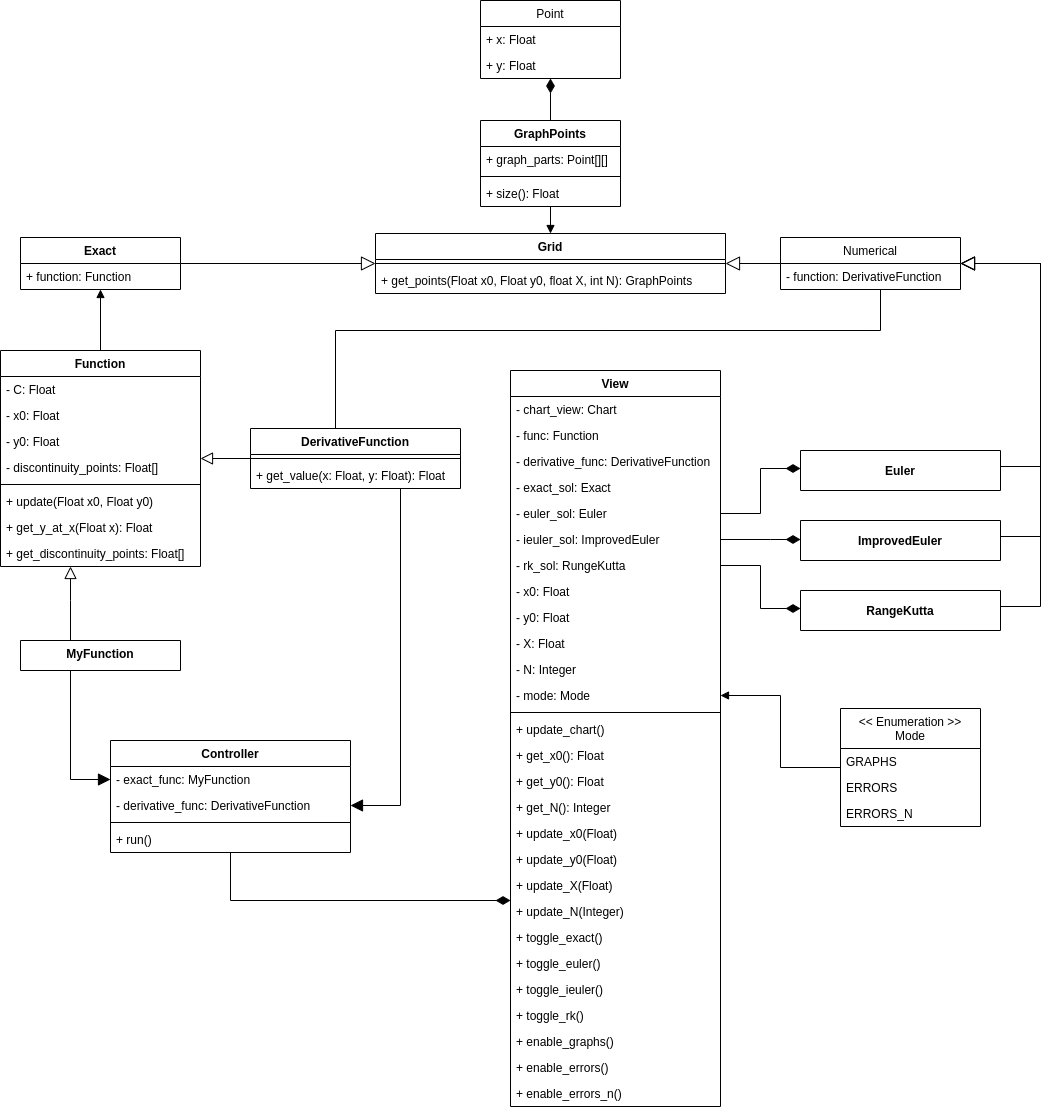
\includegraphics[scale=0.4]{resources/UML.png}
\newpage
\subsection*{Implementation}

    The program was written using the QT framework using C++. It follows 
SOLID principles and the Model-View-Controller pattern. 

The implementation includes plotting of the exact solution and numberical
solutions (Euler's method, Improved Euler's method and Runge-Kutta method),
plotting of local and average errors based on grid size, and provides control over 
variables to the user.

The following code snippet shows how the value is found for each point for Runge-Kutta method:
\begin{lstlisting}[language=C++]
    ...
    float x_prev = x;
    x += step;
    float k1 = step * function->get_value(x_prev, y);
    float k2 = step * function->get_value(x_prev + step/2, y + k1/2);
    float k3 = step * function->get_value(x_prev + step/2, y + k2/2);
    float k4 = step * function->get_value(x_prev + step, y + k3);
    y += 1.0/6.0 * (k1+2*k2+2*k3+k4);
    points.graph_parts[points.size()-1].push_back( Point(x, y) );
    ...
\end{lstlisting}

Implementation supports existance of points of discontinuity.
If the graph includes points of discontinuity, it will be split into multiple 
parts.
At each point, the function checks if it is equal or bigger than the next point 
of discontinuity, if it bigger and the current graph part has more than 0 points,
it creates a new graph part (and skips the point completely
if it is exactly equal to the point of discontinuity).

\begin{lstlisting}[language=C]
GraphPoints Exact::get_points(float x0, float y0, float X, int N){
...
    if(std::find(next_disc_pt, disc_pts.end(), x) != disc_pts.end()) {
        if ( points[points.size()-1].size() != 0 )
            points.add_graph_part();
        if ( next_disc_pt != disc_pts.end() )
            next_disc_pt++;
        continue;
    }
    else if ( x > *next_disc_pt && next_disc_pt != disc_pts.end()){
        while (x > *next_disc_pt && next_disc_pt != disc_pts.end())
            next_disc_pt++;
        if ( points[points.size()-1].size() != 0 )
            points.add_graph_part();
    }
...
\end{lstlisting}

\newpage

\subsection*{Graphs of Errors}
Program includes 3 pages: 
\begin{itemize}
\item Graphs of numerical and analytical solutions
\item Errors of each numerical method
\item Average error of each method based on step length ( controlled through N )
\end{itemize}
Each page has controls of $x_0$, $y_0$, X, N and allows the user
to choose which numerical solutions they wish to see 
(and if they wish to see the exact solution on the Graph page).

The following code snippet shows how local error is calculated for each 
part of the graph for the Euler's method:
\begin{lstlisting}[language=C++]
QLineSeries* series = new QLineSeries();
series->setName("Euler");
for (int j = 0; j < graph_points_euler[i].size(); ++j){
    float err = abs(graph_points_euler[i][j].y - graph_points_exact[i][j].y);
    series->append(graph_points_euler[i][j].x, err);
}
chartView->chart()->addSeries(series);
\end{lstlisting}

\subsection*{Miscelaneous points}
Implementation is somewhat general. For example, it is easy to replace 
the differential equation by inheriting the Function class and supplying the 
new equation to the Controller.

Some attention was paid to optimization, 
the program calculates the constant C and points of 
discontinuity only once for each x0, y0 and stores them.
Runge-Kutta implementation goes through each enabled numerical method 
in the same loop.

\subsection*{Screenshots}
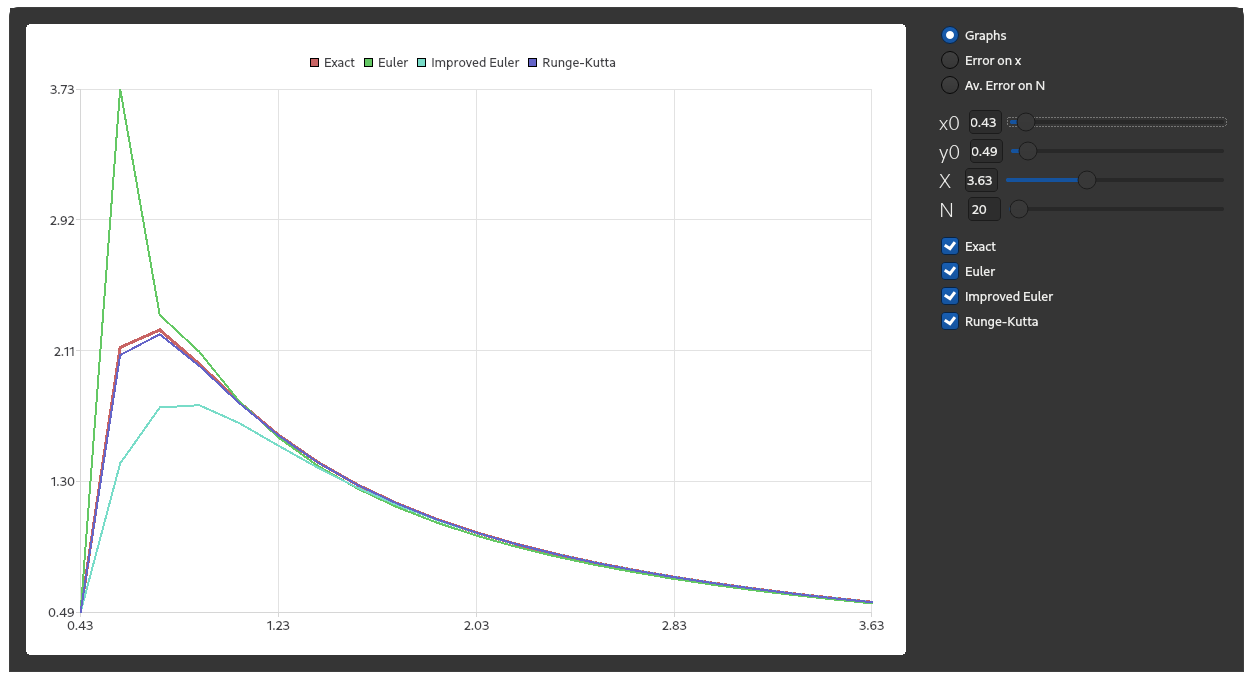
\includegraphics[scale=0.4]{resources/Screenshot1.png}
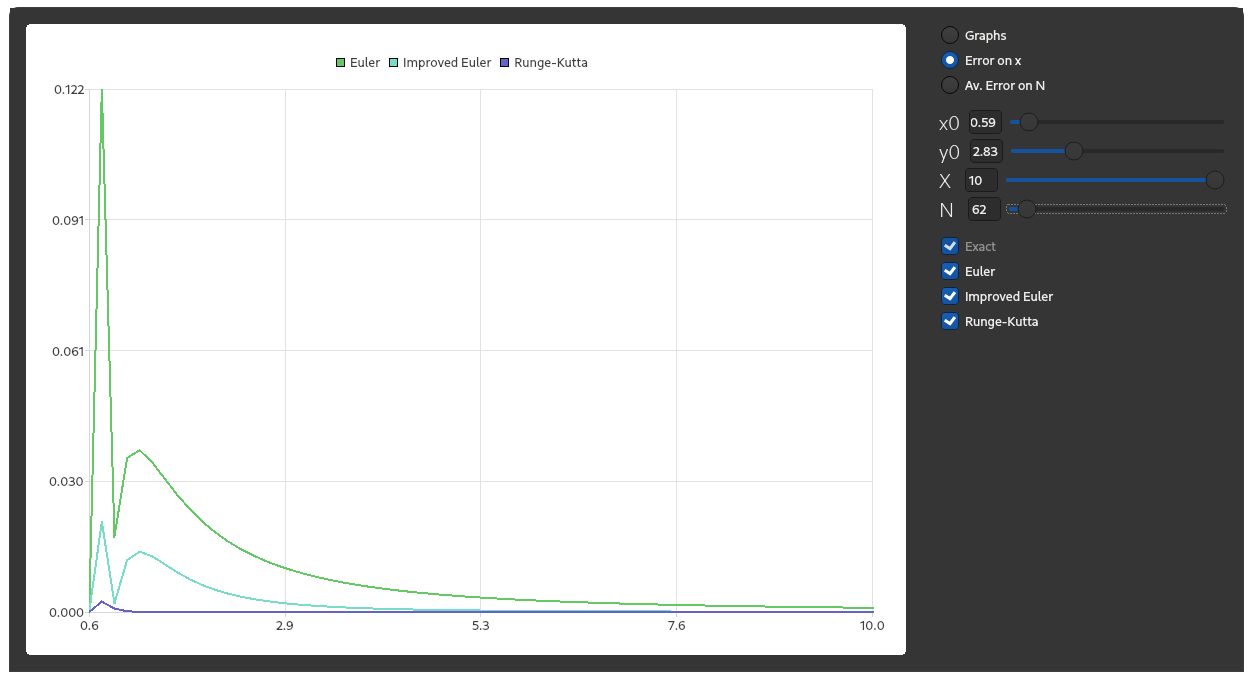
\includegraphics[scale=0.4]{resources/Screenshot2.png}
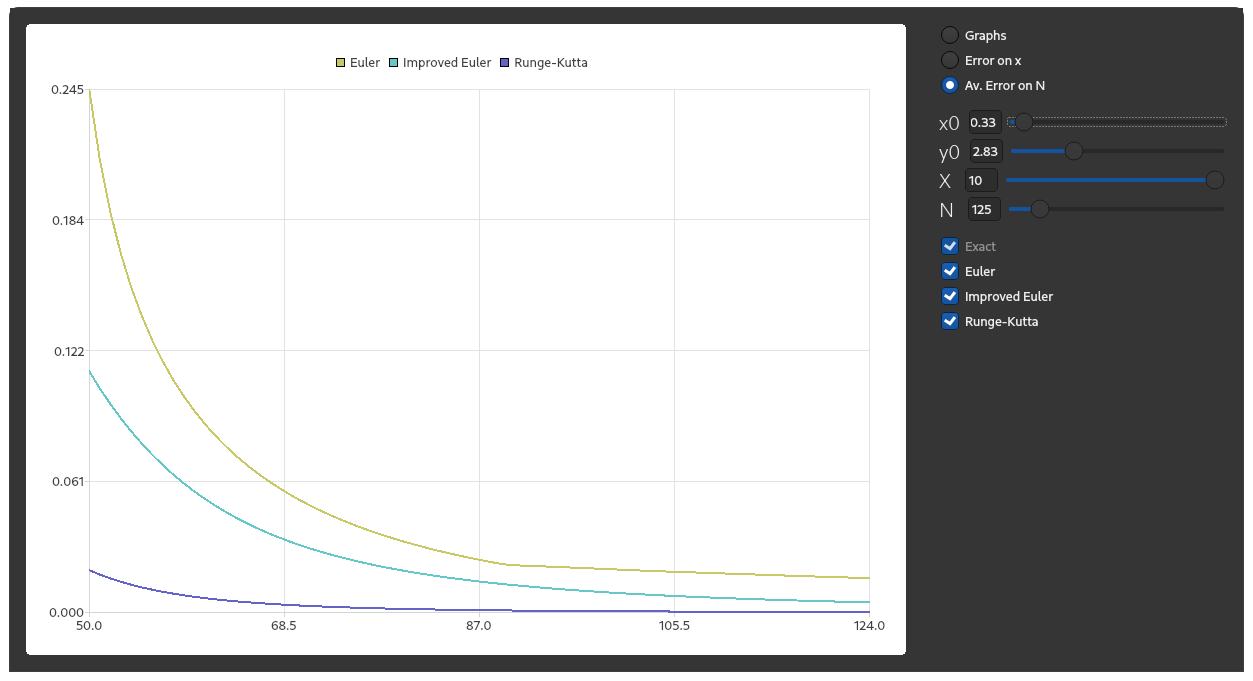
\includegraphics[scale=0.4]{resources/Screenshot3.png}
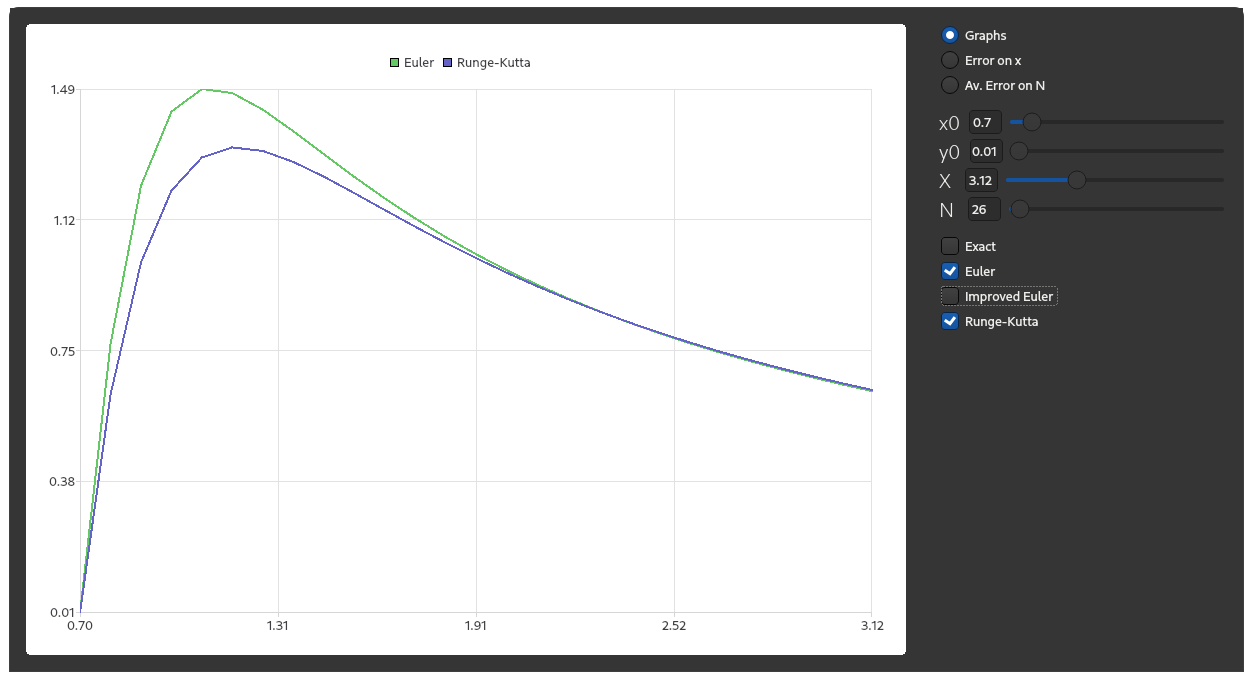
\includegraphics[scale=0.4]{resources/Screenshot4.png}


\end{document}
